\chapter{Challenges}
\section{Inherent Model Characteristics}
Although the Pix2Pix model demonstrated stable training behavior and produced high-quality image reconstructions, several challenges arose during the training process. These challenges stem from the inherent characteristics of GAN-based architectures, of which Pix2Pix is a representative example. One of the main issues encountered was the vanishing or exploding gradient problem, where the early layers of the network receive minimal updates during backpropagation, leading to slow convergence or even training stagnation. The literature attributes this behavior primarily to the choice of activation functions and optimization strategies. For instance, \cite{naderi2021} and \cite{hvt_cgan} address this issue by incorporating residual blocks to improve gradient flow. In the case of Pix2Pix, however, the vanishing gradient problem was mitigated by replacing the default binary cross-entropy (BCE) loss with the least-squares loss function. Unlike BCE, which tends to saturate when the discriminator becomes overconfident, the least-squares formulation penalizes outputs based on their squared distance from the target labels, thereby maintaining non-zero gradients even for well-classified samples~\cite{s2o_ViT_cGAN}.

Moreover, the Pix2Pix model inherently incorporates an $\mathrm{L1}$ loss term. However, a well-known limitation of the $\mathrm{L1}$ loss is that it is not well suited for generating high-resolution or perceptually rich images~\cite{s2o_ViT_cGAN}. To overcome this limitation, additional loss components based on the SSIM and the perceptual LPIPS metric were integrated into the objective function. This enhancement enabled the model to more reliably reproduce both the visual and spectral characteristics of the ground-truth multispectral images.

Another issue encountered during training was the emergence of \textit{checkerboard artifacts} in the generated images. These artifacts appeared as grid-like patterns, particularly visible in homogeneous regions such as water bodies and vegetated surfaces. The phenomenon originates from the use of transposed convolutions in the generator’s upsampling layers, where uneven overlap between convolutional kernels causes certain pixels to receive disproportionately large updates~\cite{checkerboard_deconvolution}. The same issue was also acknowledged in the official Pix2Pix implementation. To mitigate this problem, the transposed convolution layers were replaced with a combination of nearest-neighbor upsampling followed by standard convolution operations (Listing~\ref{lst:resize_conv}). This modification ensured uniform pixel coverage, effectively eliminating checkerboard artifacts and resulting in smoother and more visually coherent image reconstructions.


\begin{lstlisting}[caption={Original transposed convolution block in Pix2Pix}, label={lst:original_convtranspose}]
# Original implementation using ConvTranspose2d
nn.ConvTranspose2d(
    in_channels = ngf * mult,
    out_channels = int(ngf * mult / 2),
    kernel_size = 4,
    stride = 2,
    padding = 1,
    bias = use_bias
)
\end{lstlisting}

\begin{lstlisting}[caption={Modified resize-conv block to mitigate checkerboard artifacts}, label={lst:resize_conv}]
# Replaced with nearest-neighbor upsampling followed by regular convolution
nn.Upsample(scale_factor = 2, mode = 'bilinear'),
nn.ReflectionPad2d(1),
nn.Conv2d(
    in_channels = ngf * mult,
    out_channels = int(ngf * mult / 2),
    kernel_size = 3,
    stride = 1,
    padding = 0
)
\end{lstlisting}


\chapter{Limitaions \& Future Work}

\section{Model-Specific Limitations of GAN-Based Translation}
Despite the remarkable performance achieved by the proposed model, several limitations remain. Since the translation relies solely on SAR data, which inherently contains speckle noise, the trained model struggles to generate realistic optical images when the SAR inputs lack distinct structural information. In such cases, the model appears unable to discern meaningful spatial patterns and instead interprets some parts of the scene as noise, resulting in noise-like optical outputs, as illustrated in Figure~\ref{fig:limitation_noise}.

\begin{figure}[h!]
    \centering
    \setlength{\tabcolsep}{2pt} % horizontal padding between columns (same as ablation)
    \renewcommand{\arraystretch}{1.0} % vertical padding (same as ablation)

    \begin{tabular}{c *{3}{c}}
        % ------------------- Row 1 -------------------
        
        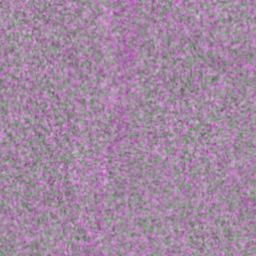
\includegraphics[width=0.2\textwidth, height=0.2\textheight, keepaspectratio]{img/limitation_noise/sample_000071_sar_pseudo.png} &
        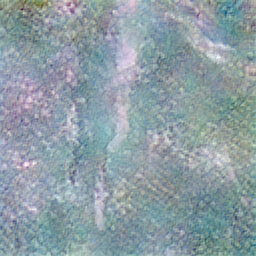
\includegraphics[width=0.2\textwidth, height=0.2\textheight, keepaspectratio]{img/limitation_noise/sample_000071_pred_rgb.png} &
        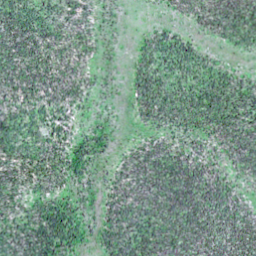
\includegraphics[width=0.2\textwidth, height=0.2\textheight, keepaspectratio]{img/limitation_noise/sample_000071_true_rgb.png} \\
        % ------------------- Row 2 -------------------
        
        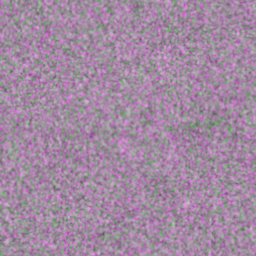
\includegraphics[width=0.2\textwidth, height=0.2\textheight, keepaspectratio]{img/limitation_noise/sample_000834_sar_pseudo.png} &
        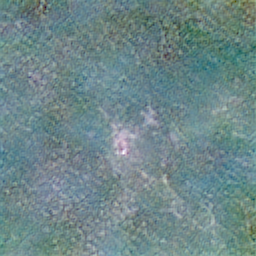
\includegraphics[width=0.2\textwidth, height=0.2\textheight, keepaspectratio]{img/limitation_noise/sample_000834_pred_rgb.png} &
        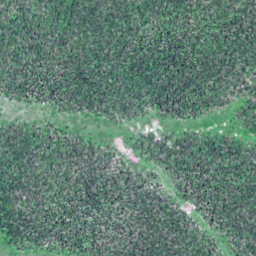
\includegraphics[width=0.2\textwidth, height=0.2\textheight, keepaspectratio]{img/limitation_noise/sample_000834_true_rgb.png} \\
    \end{tabular}

    \caption[Model limitation on structureless SAR inputs]{%
    Qualitative examples illustrating the limitation of the SAR-to-optical translation model when the SAR input lacks clear structural information. 
    Columns: 
    \textbf{(i)}~SAR input (pseudo-RGB), 
    \textbf{(ii)}~model-generated optical image, and 
    \textbf{(iii)}~reference cloud-free Sentinel-2 image. 
    }
    \label{fig:limitation_noise}
\end{figure}

This limitation suggests that future research should focus on exploring alternative generative architectures, such as Diffusion Models. Unlike GAN-based approaches, Diffusion Models learn the underlying data distribution by iteratively adding and removing noise, which often results in more stable training and higher-quality image synthesis. Furthermore, while GAN-based models are known for their instability and limited capacity to further enhance image fidelity, Diffusion Models have recently demonstrated superior performance in producing high-resolution, photorealistic outputs. Notably, the current state-of-the-art method for cloud removal on the SEN12-MS-CR dataset (see Section~\ref{sec:datasets}) is a Diffusion-based approach, namely \textit{DiffCR}~\cite{DiffCR}, underscoring the growing effectiveness of these models in handling complex remote sensing translation tasks.

\section{Temporal Generalizability Across Different Seasons}
Another important limitation lies in the model’s temporal generalizability. The Pix2Pix model was trained and evaluated primarily on the winter subset of the SEN12-MS dataset, which ensures a consistent data distribution and spectral domain during training. While the model exhibits reasonable spatial generalization when evaluated on the SEN12-MS-CR dataset—which features a distinct set of regions of interest (ROIs) compared to SEN12-MS—it struggles to maintain the same level of performance across different seasonal subsets. In particular, when applied to the summer, fall, or spring subsets, the model demonstrates a noticeable degradation in reconstruction quality, indicating sensitivity to seasonal variability in vegetation, soil moisture, and illumination conditions. Quantitative and qualitative results for the different seasons are provided in Appendix~\ref{appendix:results_seasons}.

These findings indicate that while the model performs reliably under spatial conditions similar to its training distribution, it fails to maintain consistent performance across acquisition periods with differing environmental characteristics. Future research should therefore focus on enhancing both spatial and temporal robustness. Potential strategies include domain adaptation techniques, fine-tuning with representative samples from multiple seasons and regions, and data augmentation methods that simulate seasonal and spatial variability.
